% !TEX TS-program = pdflatex
% !TEX encoding = UTF-8 Unicode

\documentclass{beamer}
% for handouts: \documentclass[handout]{beamer}

%\setbeamertemplate{background canvas}[vertical shading][bottom=white,top=structure.fg!25]
% or whatever

\usetheme[compress]{Amsterdam}
%\setbeamertemplate{headline}{}
%\setbeamertemplate{footline}{}
%\setbeamersize{text margin left=0.5cm}
  
\usepackage[english]{babel}
\usepackage{listings}
\usepackage{geometry}
\usepackage{hyperref}

\usepackage{color}
\usepackage[T1]{fontenc}
\usepackage[utf8]{inputenc}
\usepackage{lmodern}


\usepackage{tikz}
\usetikzlibrary{shapes,arrows}

\usepackage{multicol}
\lstset{
basicstyle=\scriptsize\ttfamily,
columns=flexible,
breaklines=true,
numbers=left,
%stepsize=1,
numberstyle=\tiny,
backgroundcolor=\color[rgb]{0.85,0.90,1}
}


\begin{document}

\title[Big Data and Automated Content Analysis]{\textbf{Big Data and Automated Content Analysis} \\ Week 8 -- Wednesday \\ »Looking back and froward«}
\author[Damian Trilling]{Damian Trilling \\ ~ \\ \footnotesize{d.c.trilling@uva.nl \\@damian0604} \\ \url{www.damiantrilling.net}}
\date{28 May 2018}
\institute[UvA]{Afdeling Communicatiewetenschap \\Universiteit van Amsterdam}




\tikzstyle{block} = [rectangle, draw, fill=blue!20, 
text width=5em, text centered, rounded corners, minimum height=4em]
\tikzstyle{line} = [draw]
\tikzstyle{pijltje} = [draw, -latex']
\tikzstyle{cloud} = [draw, ellipse,fill=red!20, node distance=3cm,
minimum height=2em, text width=4em, text centered,]

















\begin{frame}{}
\titlepage
\end{frame}

\begin{frame}{Today}
\tableofcontents
\end{frame}




\section{Looking back}
\subsection{Putting the pieces together}
\begin{frame}[plain]{}
Looking back\\
\textbf{Putting the pieces together}
\end{frame}


\begin{frame}{First: Our epistomological underpinnings}
	Computational Social Science
\end{frame}


\begin{frame}{Computational Social Science}
	``It is an approach to social inquiry defined by (1) the use of large, complex datasets, often—though not always— measured in terabytes or petabytes; (2) the frequent involvement of “naturally occurring” social and digital media sources and other electronic databases; (3) the use of computational or algorithmic solutions to generate patterns and inferences from these data; and (4) the applicability to social theory in a variety of domains from the study of mass opinion to public health, from examinations of political events to social movements''
	
	\vskip 0.5 cm
	\tiny{Shah, D. V., Cappella, J. N., \& Neuman, W. R. (2015). Big Data, digital media, and computational social science: Possibilities and perils. T\textit{he ANNALS of the American Academy of Political and Social Science, 659}(1), 6–13. doi:10.1177/0002716215572084}
\end{frame}





\begin{frame}{Computational Social Science}
``[\ldots] the computational social sciences employ the scientific method, complementing descriptive statistics with inferential statistics that seek to identify associations and causality. In other words, they are underpinned by an epistemology wherein the aim is to produce sophisticated statistical models that explain, simulate and predict human life.''

\vskip 0.5 cm
\tiny{Kitchin, R. (2014). Big Data, new epistemologies and paradigm shifts. \textit{Big Data \& Society, 1}(1), 1–12. doi:10.1177/2053951714528481}
\end{frame}

%
%\begin{frame}{Second: Our data}
%	content...
%\end{frame}
%
%
%
%
%\begin{frame}{Third: Our techniques}
%	content...
%	\end{frame}




\begin{frame}{Steps of a CSS project}
We learned techniques for:
\begin{itemize}
	\item retrieving data
	\item processing data
	\item analyzing data
	\item visualising data
\end{itemize}

\end{frame}

\begin{frame}[plain]
\begin{tikzpicture}[node distance = 3cm, auto]
\node [cloud] (retrieve) {retrieve};
\node [cloud, right of=retrieve] (process) {process and/or enrich};
\node [cloud, right of=process] (analyze) {analyze\\ explain\\ predict};
\node [cloud, right of=analyze] (visualize) {communi-cate};


\path [pijltje] (retrieve)--(process);
\path [pijltje] (process)--(analyze);
\path [pijltje] (analyze)--(visualize);


\node [block, below of = retrieve] (retrievetech) {files\\ APIs\\ scraping};
\node [block, below of= process] (processtech) {NLP\\ sentiment\\ LDA\\ SML};
\node [block, below of=analyze] (analyzetech) {group comparisons; statistical tests and models};
\node [block, below of=visualize] (visualizetech) {visualizations and summary tables};



\path [pijltje] (retrievetech)--(processtech);
\path [pijltje] (processtech)--(analyzetech);
\path [pijltje] (analyzetech)--(visualizetech);


\node [block, below of = retrievetech, fill=green!20] (retrievepython) {glob\\ json \& csv\\ requests\\ twitter\\ tweepy\\ lxml\\ \ldots};

\node [block, below of = processtech, fill=green!20] (processpython) {nltk\\ gensim\\ scikit-learn \ldots};

\node [block, below of = analyzetech, fill=green!20] (analyzepython) {numpy/scipy\\ pandas\\ statsmodels\\ \ldots};

\node [block, below of = visualizetech, fill=green!20] (visualizepython) {pandas\\ matplotlib\\ seaborn\\ pyldavis\\ \ldots};





\path [line, dashed] (retrieve)--(retrievetech);
\path [line, dashed] (process)--(processtech);
\path [line, dashed] (analyze)--(analyzetech);
\path [line, dashed] (visualize)--(visualizetech);



\path [line, dashed] (retrievetech)--(retrievepython);
\path [line, dashed] (processtech)--(processpython);
\path [line, dashed] (analyzetech)--(analyzepython);
\path [line, dashed] (visualizetech)--(visualizepython);
\end{tikzpicture}
\end{frame}

\subsection{A good workflow}
\begin{frame}
	A good workflow
\end{frame}




\begin{frame}{The big picture}
\begin{block}{Start with pen and paper}
\begin{enumerate}[<+->]
	\item Draw the Big Picture
	\item Then work out what components you need
\end{enumerate}
\end{block}
\end{frame}




\begin{frame}{Develop components separately}
	\begin{block}{One script for downloading the data, one script for analyzing}
		\begin{itemize}[<+->]
			\item Avoids waste of resources (e.g., unnecessary downloading multiple times)
			\item Makes it easier to re-use your code or apply it to other data
		\end{itemize}
	\end{block}
\pause
\begin{block}{Start small, then scale up}
	\begin{itemize}[<+->]
		\item Take your plan (see above) and solve \textit{one} problem at a time (e.g., parsing a review page; or getting the URLs of all review pages)
		\item (for instance, by using functions [next slides])
	\end{itemize}
\end{block}

\end{frame}	


\begin{frame}{Develop components separately}
	\begin{block}{If you copy-paste code, you are doing something wrong}
		\begin{itemize}[<+->]
			\item Write loops!
			\item If something takes more than a couple of lines, write a function!
		\end{itemize}
	\end{block}
\end{frame}

\begin{frame}[plain, fragile]
Copy-paste approach\\ (ugly, error-prone, hard to scale up)
\begin{lstlisting}
allreviews = []

response = requests.get('http://xxxxx')
tree =  fromstring(response.text)
reviewelements = tree.xpath('//div[@class="review"]')
reviews = [e.text for e in reviewelements]
allreviews.extend(reviews)

response = requests.get('http://yyyyy')
tree =  fromstring(response.text)
reviewelements = tree.xpath('//div[@class="review"]')
reviews = [e.text for e in reviewelements]
allreviews.extend(reviews)
\end{lstlisting}
\end{frame}


\begin{frame}[plain, fragile]
Better: for-loop\\ (easier to read, less error-prone, easier to scale up (e.g., more URLs, read URLs from a file or existing list)))
\begin{lstlisting}
allreviews = []

urls = ['http://xxxxx', 'http://yyyyy']

for url in urls:
    response = requests.get(url)
    tree =  fromstring(response.text)
    reviewelements = tree.xpath('//div[@class="review"]')
    reviews = [e.text for e in reviewelements]
    allreviews.extend(reviews)
\end{lstlisting}
\end{frame}




\begin{frame}[plain, fragile]
Even better: for-loop with functions\\ (main loop is easier to read, function can be re-used in multiple contexts)
\begin{lstlisting}
def getreviews(url):
    response = requests.get(url)
    tree =  fromstring(response.text)
    reviewelements = tree.xpath('//div[@class="review"]')
    return [e.text for e in reviewelements]


urls = ['http://xxxxx', 'http://yyyyy']

allreviews = []

for url in urls:
    allreviews.extend(getreviews(url))
\end{lstlisting}
\end{frame}


\begin{frame}{Scaling up}
	Until now, we did not look too much into aspects like code style, re-usability, scalability
	\begin{itemize}
		\item Use functions and classes (Appendix D.3) to make code more readable and re-usable
		\item Avoid re-calculating values
		\item Think about how to minimize memory usage (e.g., Generators, Appendix D.2)
		\item Do not hard-code values, file names, etc., but take them as arguments
	\end{itemize}	
\end{frame}




\begin{frame}{Make it robust}
You cannot foresee every possible problem.\\
Most important: Make sure your program does not fail and loose all data just because something goes wrong at case 997/1000.
	\begin{itemize}
		\item Use \texttt{try/except} to explicitly tell the program how to handle errors
		\item Write data to files (or database) in between
		\item Use \texttt{assert len(x) == len(y}) for sanity checks
	\end{itemize}	
\end{frame}


%
%
%\begin{frame}{Replicability}
%	\begin{block}{ddd}
%		\begin{enumerate}[<+->]
%			\item egjkrjhh
%		\end{enumerate}
%	\end{block}
%\end{frame}






%{\setbeamercolor{background canvas}{bg=black}
%\begin{frame}[plain]
%\makebox[\linewidth]{
%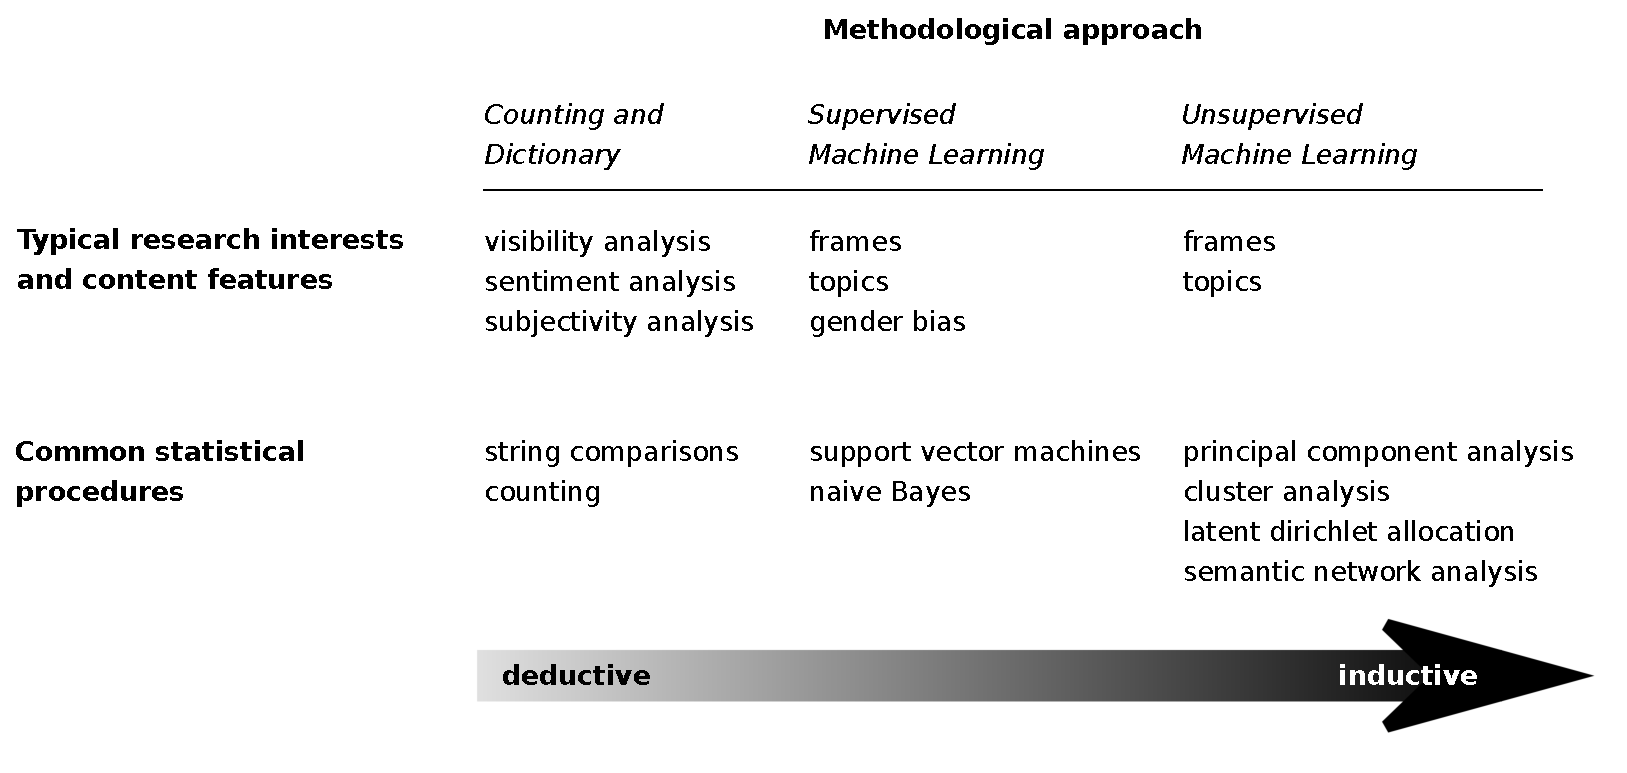
\includegraphics[width=\paperwidth,height=\paperheight,keepaspectratio]{../../pictures//boumanstrilling2016}}
%\end{frame}
%}



%
%\begin{frame}{Some terminology }
%	\begin{columns}[t]
%		\column{.5\textwidth}
%		
%		\begin{block}<1-4>{Supervised machine learning}
%			You have a dataset with both predictor and outcome (independent and dependent variables; features and labels) --- a \emph{labeled} dataset.
%			\onslide<2>{
%				\footnotesize{Think of regression: You measured \texttt{x1}, \texttt{x2}, \texttt{x3} and you want to predict \texttt{y}, which you also measured}}
%		\end{block}
%		
%		\column{.5\textwidth}
%		
%		\begin{block}<3->{Unsupervised machine learning}
%			You have no labels. \onslide<4>{(\footnotesize{You did not measure \texttt{y})}}\\
%			\onslide<5>{\textbf{Again, you already know some techniques to find out how \texttt{x1}, \texttt{x2},\ldots \texttt{x\_i} co-occur from other courses:} \begin{itemize}
%					\item Principal Component Analysis (PCA)
%					\item Cluster analysis
%					\item \ldots
%				\end{itemize}
%			}
%		\end{block}
%		
%	\end{columns}
%	
%\end{frame}
%
%



\section{Looking forward}
\subsection{Techniqes we did not cover}
\begin{frame}[plain]{}
Looking forward\\
\textbf{What other possibilities do exist for each step?}
\end{frame}


\begin{frame}[plain]
	\begin{tikzpicture}[node distance = 3cm, auto]
	\node [cloud] (retrieve) {retrieve};
	\node [cloud, right of=retrieve] (process) {process and/or enrich};
	\node [cloud, right of=process] (analyze) {analyze\\ explain\\ predict};
	\node [cloud, right of=analyze] (visualize) {communi-cate};
	
	
	\path [pijltje] (retrieve)--(process);
	\path [pijltje] (process)--(analyze);
	\path [pijltje] (analyze)--(visualize);
	
	
	\node [block, below of = retrieve] (retrievetech) {?};
	\node [block, below of= process] (processtech) {?};
	\node [block, below of=analyze] (analyzetech) {?};
	\node [block, below of=visualize] (visualizetech) {?};
	
	
	
	\path [pijltje] (retrievetech)--(processtech);
	\path [pijltje] (processtech)--(analyzetech);
	\path [pijltje] (analyzetech)--(visualizetech);
	
	
	\node [block, below of = retrievetech, fill=green!20] (retrievepython) {?};
	
	\node [block, below of = processtech, fill=green!20] (processpython) {?};
	
	\node [block, below of = analyzetech, fill=green!20] (analyzepython) {?};
	
	\node [block, below of = visualizetech, fill=green!20] (visualizepython) {?};
	
	
	
	
	
	\path [line, dashed] (retrieve)--(retrievetech);
	\path [line, dashed] (process)--(processtech);
	\path [line, dashed] (analyze)--(analyzetech);
	\path [line, dashed] (visualize)--(visualizetech);
	
	
	
	\path [line, dashed] (retrievetech)--(retrievepython);
	\path [line, dashed] (processtech)--(processpython);
	\path [line, dashed] (analyzetech)--(analyzepython);
	\path [line, dashed] (visualizetech)--(visualizepython);
	\end{tikzpicture}
\end{frame}



\begin{frame}{Retrieve}
	\begin{block}{Webscraping with Selenium}
	\begin{itemize}
		\item 	If content is dynamically loaded (e.g., with JavaScript), our approach doesn't work (because we don't have a browser).
		\item 	Solution: Have Python literally open a browser and literally click on things
		\item $\Rightarrow$ Appendix E
	\end{itemize}
	\end{block}
\end{frame}



\begin{frame}{Retrieve}
	\begin{block}{Use of databases}
	We did not discuss how to actually store the data
	\begin{itemize}
		\item We basically stored our data in files (often, one CSV or JSON file)
		\item But that's not very efficient if we have large datasets; especially if we want to select subsets later on
		\item SQL-databases to store tables (e.g., MySQL)
		\item NoSQL-databases to store less structured data (e.g., JSON with unknown keys) (e.g., MongoDB, ElasticSearch)
		\item $\Rightarrow$ \tiny{Günther, E., Trilling, D., \& Van de Velde, R.N. (2018). But how do we store it? (Big) data architecture in the social-scientific research process. In:\textit{ Stuetzer, C.M., Welker, M., \& Egger, M. (eds.): Computational Social Science in the Age of Big Data. Concepts, Methodologies, Tools, and Applications}. Cologne, Germany: Herbert von Halem.}
	\end{itemize}
	\end{block}
\end{frame}





\begin{frame}{Storing data}
	\makebox[\linewidth]{
		\includegraphics[width=\paperwidth,height=\paperheight,keepaspectratio]{../../pictures/guenteretal_fig1}}
\end{frame}




\begin{frame}{From retrieved data to enriched data}
	\makebox[\linewidth]{
		\includegraphics[width=\paperwidth,height=\paperheight,keepaspectratio]{../../pictures/guentheretal_fig3}}
\end{frame}




\begin{frame}{Process and/or enrich}
	\begin{block}{Word embeddings}
	We did not really consider the \emph{meaning} of words
		\begin{itemize}
		\item Word embeddings can be trained on large corpora (e.g., whole wikipedia or a couple of years of newspaper coverage) 
		\item The trained model allows you to calculate with words (hence, word vectors): $king-man+woman = ?$ 
		\item You can find out whether documents are similar \emph{even if they do not use the same words} (Word Mover Distance)
		\item $\Rightarrow$ word2vec (in gensim!), glove
		\end{itemize}
	\end{block}
\end{frame}





\begin{frame}{Process and/or enrich}
	\begin{block}{Advanced NLP}
		We did a lot of BOW (and some POS-tagging), but we can get more
		\begin{itemize}
			\item Named Entity Recognition (NER) to get names of people, organizations, \ldots
			\item Dependency Parsing to find out exact relationships
			$\Rightarrow$ nltk, Stanford, FROG. And now (that one is really cool): spacy
		\end{itemize}
	\end{block}
\end{frame}



\begin{frame}{Process and/or enrich}
\begin{block}{Use images}
\begin{itemize}
	\item  Supervised Machine learning does not care about what the features mean, so instead of texts we can also classify pictures
	%\item  Based on a pre-coded training set, the computer compares images sorted into two (or more) groups
	\item  Example: Teach the computer to decide whether an avatar on a social medium is an actual photograph of a person or a drawn image of something else (research Marthe)
	\item  This principle can be applied to many fields and disciplines -- for example, it is possible to teach a computer to indicate if a tumor is present or not on X-rays of people's brains
\end{itemize}
\end{block}
\end{frame}


\begin{frame}{Process and/or enrich}
	\begin{block}{Use images}
		\begin{itemize}
	\item To learn more about this, the following websites useful information: \url{http://blog.yhat.com/posts/image-classification-in-Python.html} and \url {http://cs231n.github.io/python-numpy-tutorial/\#numpy-arrays}
	\item Possibible workflow: Pixel color values as features $\Rightarrow$ PCA to reduce features  $\Rightarrow$ train classifier
	\item Advanced stuff: Neural Networks
\end{itemize}
	\end{block}
\end{frame}


\begin{frame}{Analyze/explain/predict}
	\begin{block}{More advanced modelling}
We only did some basic statistical tests
		\begin{itemize}
			\item Especially with social media data, we often have time series (VAR models etc.)
			\item There are more advanced regression techniques and dimension-reduction techniques tailored to data that are, e.g., large-scale, sparse, have a lot of features, \ldots
		\item $\Rightarrow$ scikit-learn, statsmodels
		\end{itemize}
	\end{block}
\end{frame}










\section{The INCA project}
\subsection{Scaling up Content Analyis}
\begin{frame}[plain]{}
An example for scaling up:\\
\textbf{The INCA project}
\vskip 3cm
\small{see also Trilling, D., \& Jonkman, J.G.F. (2018). Scaling up content analysis. \textit{Communication Methods and Measures}, doi:10.1080/19312458.2018.1447655}
\end{frame}



\begin{frame}[plain]
	\makebox[\linewidth]{
		\includegraphics[width=\paperwidth,height=\paperheight,keepaspectratio]{../../pictures/scalingup2}}
\end{frame}


\begin{frame}{INCA}
\begin{block}{How do we move beyond one-off projects?}
	\begin{itemize}
		\item Collect data in such a way that it can be used for multiple projects
		\item Database backend
		\item Re-usability of preprocessing and analysis code
	\end{itemize}
\end{block}
\end{frame}



\begin{frame}{INCA}
	\begin{block}{The idea}
		\begin{itemize}
		\item Usable with minimal Python knowledge
		\item The ``hard stuff'' is already solved: writing a scraper often only involves replacing the XPATHs
		\end{itemize}
	\end{block}
\end{frame}




\subsection{The INCA architecture}

\begin{frame}[plain]
	\makebox[\linewidth]{
		\includegraphics[width=\paperwidth,height=\paperheight,keepaspectratio]{../../pictures/scalingup1}}
\end{frame}


\begin{frame}[plain]
\makebox[\linewidth]{
	\includegraphics[width=\paperwidth,height=\paperheight,keepaspectratio]{../../pictures/inca1}}
\end{frame}


\begin{frame}[plain]
	\makebox[\linewidth]{
		\includegraphics[width=\paperwidth,height=\paperheight,keepaspectratio]{../../pictures/inca2}}
\end{frame}






\section{Final steps}

\begin{frame}{Next meeting}
\begin{block}{Friday}
	Final chance for questions regarding final project (if you don't have any, you don't need to come.)
\end{block}

\begin{block}{Deadline final exam}
Hand in via filesender until Sunday evening, 23.59.\\
One .zip or .tar.gz file with
\begin{itemize}
	\item .py and/or .ipynb for code
	\item .pdf for text and figures
	\item .csv, .json, or .txt for data
	\item any additional file we need to understand or reproduce your work
\end{itemize}
\end{block}

\end{frame}




\end{document}

